%---------- Inleiding ---------------------------------------------------------

\section{Introductie}%
\label{sec:introductie}

In dit onderzoeksvoorstel, uitgevoerd bij ILVO, worden geavanceerde mogelijkheden van technologieën verkend voor het volgen en begrijpen van koeiengedrag in de moderne veehouderij. 
Het correct volgen en identificeren van gedrag van koeien is van cruciaal belang, niet alleen voor het welzijn van de dieren, maar ook voor de operationele efficiëntie van boerderijen. 
Deze studie richt zich op het analyseren van verschillende technologische methoden, waaronder objectdetectie en diepteschatting, om de locatie van koeien te bepalen en gedragingen zoals grazen, wandelen en rusten te identificeren. We onderzoeken de praktische uitdagingen en kansen die deze technologieën bieden in een agrarische omgeving. 
Het doel is om een diepgaand inzicht te krijgen in hoe deze technologische vooruitgang kan leiden tot verbeteringen in veehouderijpraktijken, met een specifieke focus op de impact op dierenwelzijn en boerderijbeheer. 
Dit onderzoek zal niet alleen bijdragen aan de wetenschappelijke kennis over diergedrag en technologische toepassingen in de landbouw, maar ook praktische richtlijnen bieden voor implementatie in de sector, wat de weg vrijmaakt voor innovatieve oplossingen in de toekomst van de landbouw.
%---------- Stand van zaken ---------------------------------------------------

\section{Literatuurstudie}%
\label{sec:state-of-the-art}
De technologische vooruitgang in de veehouderij heeft een nieuwe dimensie toegevoegd aan het volgen en analyseren van vee. 
De integratie van GPS- en RFID-technologieën, zoals onderzocht door \autocite{Nääs2013}\autocite{Akhigbe2021}, heeft de basis gelegd voor efficiëntere trackingmethoden. 
Deze technologieën spelen een cruciale rol in het bieden van inzicht in de bewegingen en het gedrag van vee, wat essentieel is voor het beheer van hun gezondheid en welzijn.
Ontwikkelingen in computervisie en machine learning hebben nieuwe mogelijkheden geopend voor real-time monitoring en gedragsanalyse, zoals benadrukt door \autocite{Kleanthous2018}. 
Geavanceerde technieken zoals objectdetectie en keypoints-analyse bieden gedetailleerde inzichten in het gedrag van vee, wat van groot belang is voor hun welzijnsbeoordeling. 
De toepassing van 3D-beeldvormings-technologieën, onderzocht \\door \autocite{LeCozler2019}, heeft de precisie in het volgen en analyseren van vee verder verhoogd.
Deze methoden stellen ons in staat om gedetailleerde informatie te verzamelen, wat cruciaal is voor het beoordelen van de fysieke gezondheid van het vee.
Echter brengen deze ontwikkelingen ook uitdagingen met zich mee, zoals het identificeren van gedrag in verschillende omgevingscondities en het handhaven van nauwkeurigheid in complexe landbouwomgevingen \autocite{Narayan2023}\autocite{Busse2015}. 
Het is belangrijk om een evenwicht te vinden tussen het gebruik van geavanceerde technologieën en het waarborgen van dierenwelzijn en duurzaamheid.
Deze studies onderstrepen de vooruitgang en de voortdurende behoefte aan onderzoek en ontwikkeling in de implementatie en effectiviteit van technologieën. 
De integratie van deze technologieën belooft een efficiënte en diergerichte toekomst voor de veehouderij.
%---------- Methodologie ------------------------------------------------------
\section{Methodologie}%
\label{sec:methodologie}
Fasen van het onderzoek:
\begin{itemize}
  \item Fase 1: Literatuurstudie (1 week)
  \item Fase 2: Datacollectie (2 weken)
  \item Fase 3: Technologieën en Technieken (3 weken)
  \item Fase 4: Data-analyse en -verwerking (4 weken)
  \item Fase 5: Integratie en Evaluatie (2 weken)
  \item Fase 6: Conclusie (2 weken)
\end{itemize}
\subsection{Literatuurstudie}
Deze fase richt zich op het verkrijgen van een kennis van de huidige stand van zaken in de technologieën voor vee tracking. 
De focus ligt op het analyseren van studies over machine learning en computervisie. 
Hierbij is het doel het identificeren van de meest effectieve methoden en technieken voor gedragsanalyse van vee.
\end{itemize}
\subsection{Datacollectie}
In deze fase wordt real-time gedragsdata van koeien verzameld met behulp van camera's. 
Het doel is om een efficiënt systeem voor data-extractie en -beheer te ontwikkelen, evenals het opzetten van geautomatiseerde data pipelines. 
Daarnaast zal onderzocht worden over welke soortgelijke technologieën ILVO reeds beschikt en en of er bestaande ILVO-datasets zijn die gebruikt kunnen worden. 
Dit zal helpen bij het verrijken en uitbreiden van de verzamelde data.
\end{itemize}
\subsection{Technologieën en Technieken}
Selectie en integratie van de meest geschikte technologieën voor de analyse van koeiengedrag. 
Dit omvat de aanpassing van bestaande computervisietechnieken zoals objectdetectie en keypoints-analyse.
\end{itemize}
\subsection{Data-analyse en -verwerking}
Grondige analyse en classificatie van koeiengedrag uit de verzamelde data. 
Toepassing van geavanceerde machine learning algoritmen en patroonherkenning voor diepgaande analyse. 
De focus ligt op het voorverwerken van data, het trainen van modellen en het valideren van resultaten.
\end{itemize}
\subsection{Integratie en Evaluatie}
Implementatie en toetsing van de ontwikkelde technieken en modellen in een realistische landbouwomgeving. 
Beoordeling van de effectiviteit, nauwkeurigheid en bruikbaarheid van de technologieën. 
\subsection{Conclusie}
Reflectie op de resultaten van het onderzoek, met een nadruk op de impact van de geïntegreerde technologieën en methoden op de veehouderijpraktijk. 
Aanbevelingen voor toekomstig onderzoek en mogelijke verbeteringen.
\subsection{Gantt-chart}
\newline
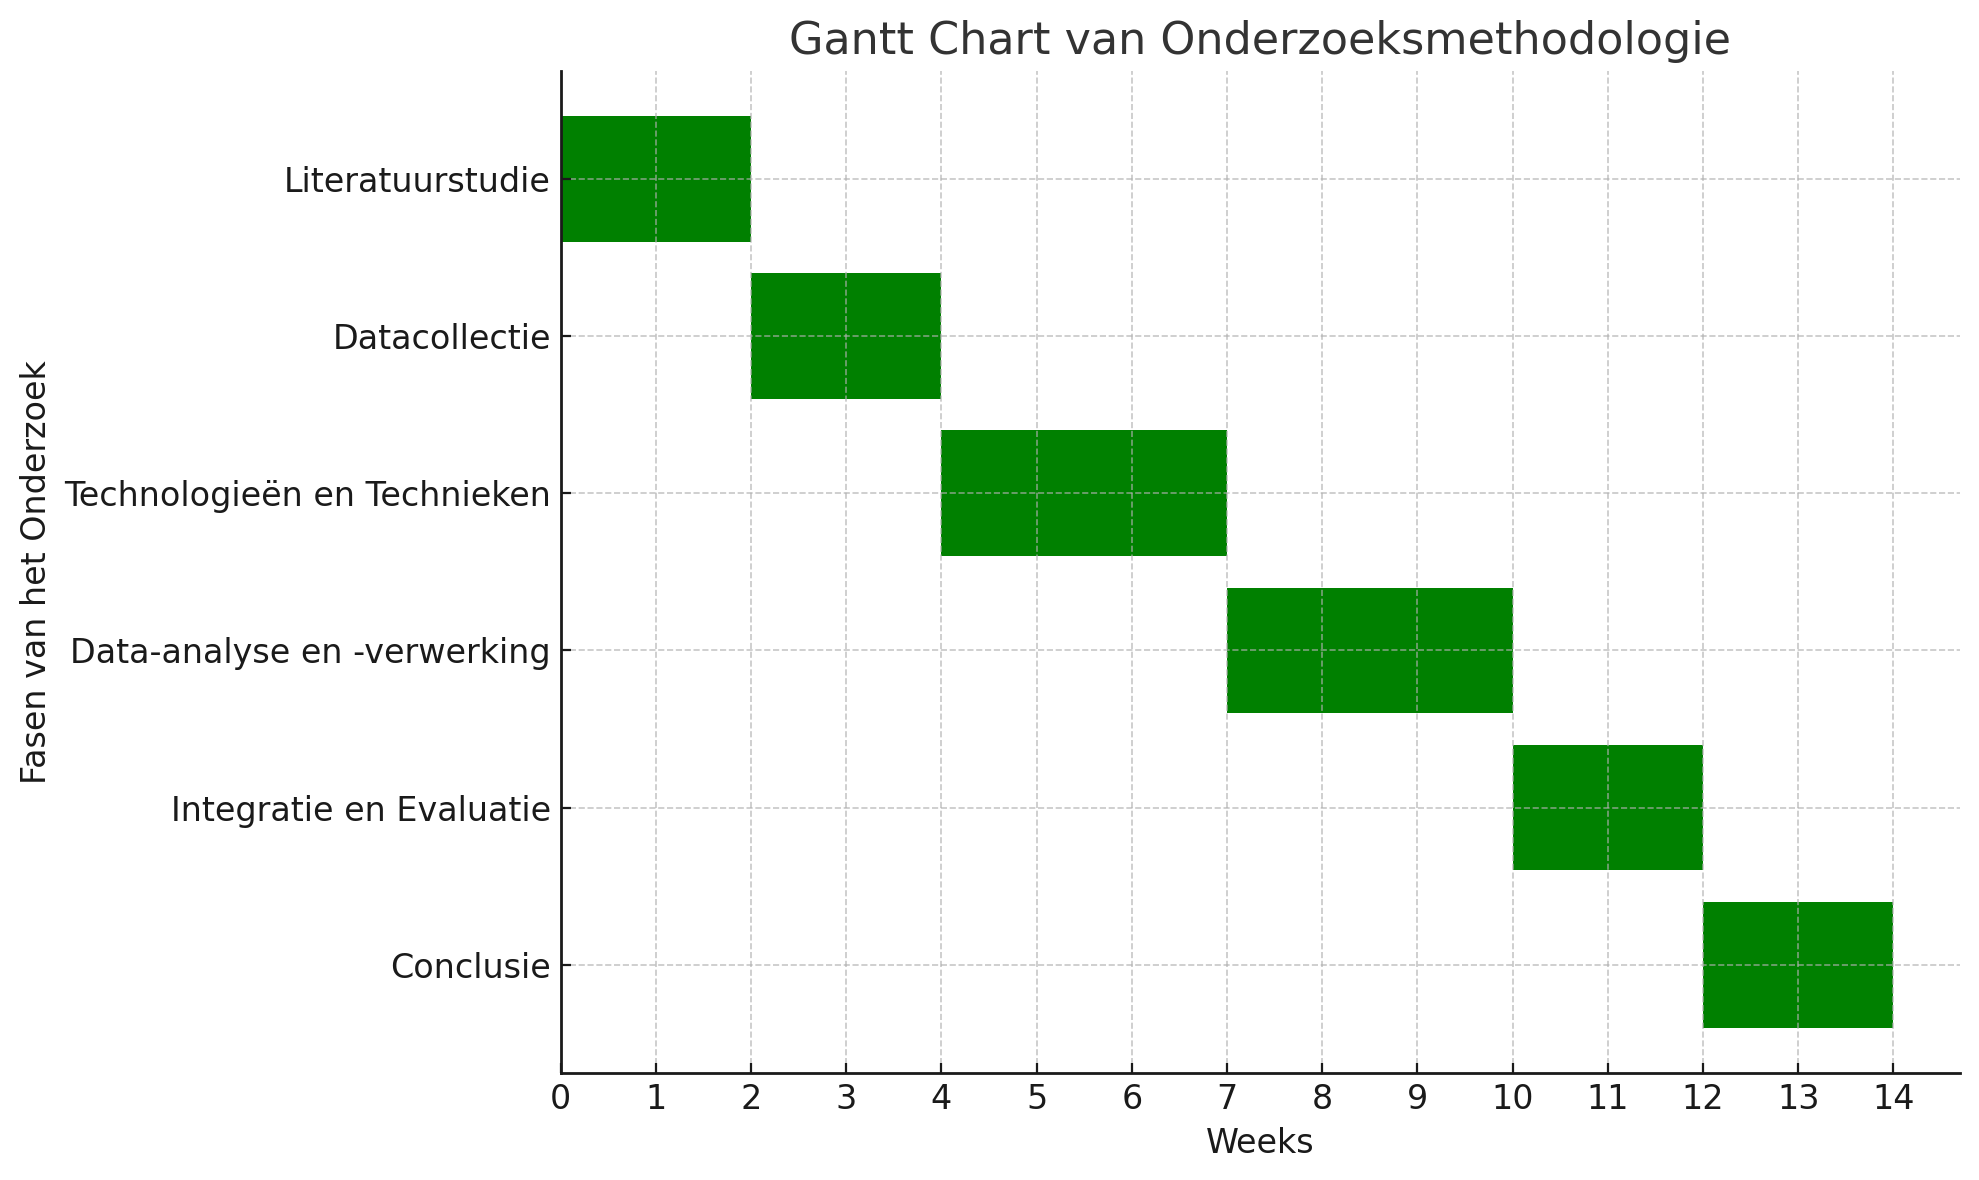
\includegraphics[width=\linewidth]{gantt_chart.png}
\newline
%---------- Verwachte resultaten ----------------------------------------------
\section{Verwacht resultaat, conclusie}%
\label{sec:verwachte_resultaten}
In dit onderzoek verwachten we de volgende resultaten te verkrijgen:
\begin{itemize}
  \item Verbeterde nauwkeurigheid in het monitoren van koeiengedrag door geavanceerde technologieën, zoals objectdetectie en \newline keypoints-analyse, toe te passen.
  \item Efficiëntere methoden voor gedragsanalyse van koeien in verschillende omgevingsomstandigheden.
  \item Een geïntegreerd systeem dat zowel de locatie als het gedrag van koeien kan volgen en nauwkeurige gegevens kan genereren.
\end{itemize}
Deze resultaten zullen een meerwaarde bieden voor de veehouderij door bij te dragen aan het welzijn van dieren en de operationele efficiëntie te verbeteren. Het gebruik van geavanceerde technologieën voor gedragsmonitoring kan leiden tot betere besluitvorming en zorg voor het vee, en uiteindelijk tot positieve economische en ethische gevolgen voor de landbouwsector.

Het is belangrijk op te merken dat de uiteindelijke resultaten kunnen variëren op bas
is van de uitkomsten van de data-analyse en evaluatie van de gebruikte technologieën. Dit onderzoek zal een grondige analyse bieden om eventuele afwijkingen te verklaren en aanbevelingen te doen voor verdere verbeteringen.
